\documentclass{article}
\usepackage[utf8]{inputenc}
\usepackage{t1enc}
\usepackage{geometry}
 \geometry{
 a4paper,
 total={210mm,297mm},
 left=20mm,
 right=20mm,
 top=20mm,
 bottom=20mm,
 }
\usepackage{amsmath}
\usepackage{amssymb}
\usepackage{pgf,tikz}
\usetikzlibrary{arrows}
\usetikzlibrary{patterns}
\frenchspacing
\usepackage{fancyhdr}
\pagestyle{fancy}
\lhead{Urbán János tanár úr feladatsorai}
\chead{C08/7-8. osztály}
\rhead{Szakkör}
\lfoot{}
\cfoot{\thepage}
\rfoot{}

\usepackage{enumitem}
\usepackage{multicol}
\usepackage{calc}
\newenvironment{abc}{\begin{enumerate}[label=\textit{\alph*})]}{\end{enumerate}}
\newenvironment{abc2}{\begin{enumerate}[label=\textit{\alph*})]\begin{multicols}{2}}{\end{multicols}\end{enumerate}}
\newenvironment{abc3}{\begin{enumerate}[label=\textit{\alph*})]\begin{multicols}{3}}{\end{multicols}\end{enumerate}}
\newenvironment{abc4}{\begin{enumerate}[label=\textit{\alph*})]\begin{multicols}{4}}{\end{multicols}\end{enumerate}}
\newenvironment{abcn}[1]{\begin{enumerate}[label=\textit{\alph*})]\begin{multicols}{#1}}{\end{multicols}\end{enumerate}}
\setlist[enumerate,1]{listparindent=\labelwidth+\labelsep}

\newcommand{\degre}{\ensuremath{^\circ}}
\newcommand{\tg}{\mathop{\mathrm{tg}}\nolimits}
\newcommand{\ctg}{\mathop{\mathrm{ctg}}\nolimits}
\newcommand{\arc}{\mathop{\mathrm{arc}}\nolimits}
\renewcommand{\arcsin}{\arc\sin}
\renewcommand{\arccos}{\arc\cos}
\newcommand{\arctg}{\arc\tg}
\newcommand{\arcctg}{\arc\ctg}

\parskip 8pt
\begin{document}

\section*{Szakkör}

\subsection*{2008.09.30.}
\begin{enumerate}
\item Keressünk három olyan számot, amelyik 9-jegyű, minden 0-tól különböző számjegy pontosan egyszer szerepel mindegyikben és két szám összege a harmadik.
\item Hány olyan csupa különböző számjegyekből álló ötjegyű szám van, amelyben a 
számjegyek csökkenő sorrendben állnak?
\item Adott öt szám. Ezekből képeztük az összes lehetséges háromtagú összeget. 
A következő összegeket kaptuk: $3,4,6,7,9,10,11,14,15$ és $17$. Mi volt a kiindulásul választott öt szám?
\item Egy háromszög egyik belső szöge $60^\circ$-os, a szöget közrefogó oldalai pedig 2 és 3 egység hosszúak. Daraboljuk fel a háromszöget szakaszokkal három részre úgy, hogy a részekből egy szabályos hatszöget lehessen össze\-rakni.
\item Adjunk meg 2009 darab (nem feltétlenül különböző) pozitív egész számot úgy, 
hogy az összegük egyenlő legyen a szorzatukkal. 
\end{enumerate}

\subsection*{2008.10.07.}
\begin{enumerate}
\item A 0-tól különböző számjegyekből álló $S$ halmazt fel lehet-e bontani két részhalmazra úgy, hogy egyikre se legyen igaz a következő tulajdonság:
\textit{a részhalmaz két elemmel együtt tartalmazza azok különbségét is}?
\item Egy kockát mind a hat lapjára tükrözünk. Az eredeti kockával együtt így egy új testet kapunk. Hányszorosa a kapott test felszíne az eredeti kocka felszínének?
\item 14 különböző pozitív egész szám összege 110. Melyek ezek a számok?
\item A pozitív egész számokat felírtuk egy nagy papírra 1-től 10~000-ig, ezután kihúztuk azokat, amelyekben szerepel a 0 vagy a 9 számjegy. Hány szám maradt?
\item Egy szabályos hatszög minden oldalát öt egyenlő részre osztottuk. Hány olyan 
háromszög van, amelynek csúcsai az így kapott osztópontok közül kerülnek ki?
\end{enumerate}

\subsection*{2008.10.14.}
\begin{enumerate}
\item Igazoljuk, hogy az
$$1+2+3+4+\ldots+n$$
összeg értékének tízes számrendszerbeli alakjában az egyesek helyén álló számjegy periodikusan ismétlődik.
\item Igazoljuk, hogy 11 pozitív egész szám között mindig van kettő, amelyek különbsége osztható 10-zel!
\item Adott a síkon húsz pont. Ezek közül bizonyos pontpárokat összekötöttünk szakaszokkal. Igazoljuk, hogy mindig van a 20 pont között kettő olyan, amelyekből azonos számú szakasz indul ki.
\item Egy ötemeletes házat hányféleképpen tudunk kifesteni, ha minden emeletet vagy fehérre, vagy zöldre festhetnek, de két fehér emelet nem kerülhet egymás felé? Oldjuk meg a feladatot 6, 7, 8 emeletes házra is!
\item Egy paralelogramma egyik átlóján kiválasztottunk egy pontot és ezen át párhuzamosokat húztunk az oldalakkal. 

\centerline{
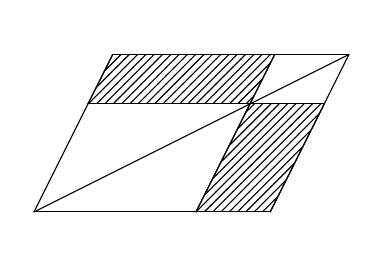
\begin{tikzpicture}[line cap=round,line join=round,>=triangle 45,x=1.0cm,y=1.0cm]
\clip(-0.08000000000000056,-0.24000000000000235) rectangle (4.119999999999999,2.3399999999999985);
\fill[fill=black,pattern=north east lines,pattern color=black] (0.6859999999999999,1.3719999999999999) -- (2.7439999999999998,1.3719999999999999) -- (3.058,2.0) -- (1.0,2.0) -- cycle;
\fill[fill=black,pattern=north east lines,pattern color=black] (2.7439999999999998,1.3719999999999999) -- (2.058,-0.0) -- (3.0,0.0) -- (3.686,1.3719999999999999) -- cycle;
\draw (0.0,0.0)-- (3.0,0.0);
\draw (3.0,0.0)-- (4.0,2.0);
\draw (4.0,2.0)-- (1.0,2.0);
\draw (1.0,2.0)-- (0.0,0.0);
\draw (0.0,0.0)-- (4.0,2.0);
\draw (0.6859999999999999,1.3719999999999999)-- (3.686,1.3719999999999999);
\draw (3.058,2.0)-- (2.058,-0.0);
\draw (0.6859999999999999,1.3719999999999999)-- (2.7439999999999998,1.3719999999999999);
\draw (2.7439999999999998,1.3719999999999999)-- (3.058,2.0);
\draw (3.058,2.0)-- (1.0,2.0);
\draw (1.0,2.0)-- (0.6859999999999999,1.3719999999999999);
\draw (2.7439999999999998,1.3719999999999999)-- (2.058,-0.0);
\draw (2.058,-0.0)-- (3.0,0.0);
\draw (3.0,0.0)-- (3.686,1.3719999999999999);
\draw (3.686,1.3719999999999999)-- (2.7439999999999998,1.3719999999999999);
\end{tikzpicture}
}

\noindent Igazoljuk, hogy a besatírozott két kis paralelogramma területe egyenlő!
\end{enumerate}

\subsection*{2008.11.11.}
\begin{enumerate}
\item Igazoljuk, hogy bármely 11 darab pozitív egész szám közül kiválasztható néhány (esetleg egy, de lehet, hogy az összes), amelyek összege osztható 11-gyel! 
\item Melyik az a legkisebb pozitív egész szám, amely 2-vel, 3-mal, 4-gyel, 5-tel és 6-tal osztva mindig 1 maradékot ad és 7-tel osztható?
\item A 4-es és 5-ös számjegyekből hány olyan 8-jegyű számot képezhetünk, amelyben a 4-esek és 5-ösök száma egyenlő?
\item Adott a síkon 25 pont, amelyek közül semelyik 3 nem esik egy egyenesbe. Hány háromszöget határoznak meg?
\item Hány átlója van egy konvex húszszögnek? 
\item Rajzoltunk a síkon 11 egyenest úgy, hogy nincs köztük 2, ami párhuzamos lenne. Igazoljuk, hogy kiválaszt\-ha\-tó közülük 2 olyan, amelyek $17^\circ$-nál kisebb szöget zárnak be.
\item Az $ABCDEFGH$ szabályos nyolcszög területének hányad része az $ABEF$ téglalap területe?
\item Adott a síkon 5 pont úgy, hogy semelyik három nincs egy egyenesen. Minden pontot összekötünk a többi 4 pont mindegyikével. Kiszínezhetők-e a kapott szakaszok 4 színnel úgy, hogy minden csúcsból 4 különböző színű szakasz indul ki?
\end{enumerate}

\subsection*{2008.11.25.}
\begin{enumerate}
\item Melyek azok a $p$ prímszámok, amelyekre $2p-1$, és $2p+1$ is prímszám?
\item Az első 100 pozitív egész számot fel lehet-e osztani két csoportra úgy, hogy a csoportokba tartozó számok összege egyenlő legyen?\\
És úgy, hogy a szorzatuk egyenlő legyen?
\item Hányféleképpen választhatunk ki két 1 és 20 közötti egész számot úgy, hogy az összegük páratlan legyen?
\item Hányféleképpen választhatunk ki 10 különböző könyv közül páratlan számút?
\item Az első 90 pozitív egész szám közül hányféleképpen választhatunk ki 3-mat úgy, hogy a számok összege osztható legyen hárommal?
\item Igazoljuk, hogy egy négyzet feldarabolható bármely 5-nél nagyobb számú (nem feltétlenül egybevágó) négyzetre.
\item Egy háromszög egyik szöge $68^\circ$. Mekkora szöget zár be a másik két szög szögfelezője?
\end{enumerate}

\subsection*{2009.01.20.}
\begin{enumerate}
\item Hány olyan ötjegyű pozitív egész szám van, amelyben van 8-as és 9-es számjegy is? 
\item Határozzuk meg az összes $\overline{aabb}$ alakú négyzetszámot.
\item Igazoljuk, hogy két 9-re végződő természetes szám négyzetének különbsége osztható 40-nel.
\item ($*$) Mennyi maradékot kapunk, ha a $2008^{2009}+2009^{2008}$ összeget
osztjuk $2008\cdot 2009$-cel?
\item Egy papírlapot 10 részre vágunk, majd az így kapott részek közül néhányat újra 10 részre vágunk és így tovább. Kaphatunk-e végül ezzel az eljárással 2009 
papírdarabot?
\end{enumerate}

\subsection*{2009.01.07.}
\begin{enumerate}
\item Hány olyan hatjegyű szám van, amely csak az 1, 2, 3 számjegyeket tartalmazza,
mindegyiket legalább egyszer?
\item Hány olyan különböző számjegyekből álló négyjegyű szám van, amelyben két páros és két páratlan számjegy szerepel?
\item Számítsuk ki azoknak az ötjegyű számoknak az összegét, amelyeknek mindegyik számjegye páratlan.
\item Hány átlója van egy konvex húszszögnek?
\item Egy konvex sokszögbe összesen 77 átló húzható. Hány oldalú a sokszög?
\item Egy társaságban mindenki mindenkivel kezet fogott. Hányan voltak a társaságban, ha összesen 136 kézfogás volt?
\end{enumerate}

\subsection*{2008.02.10.}
\begin{enumerate}
\item Egy négyzetrácsos papíron megrajzoltuk az ábrán látható szögeket.

\smallskip
\centerline{
\definecolor{qqqqff}{rgb}{0.0,0.0,1.0}
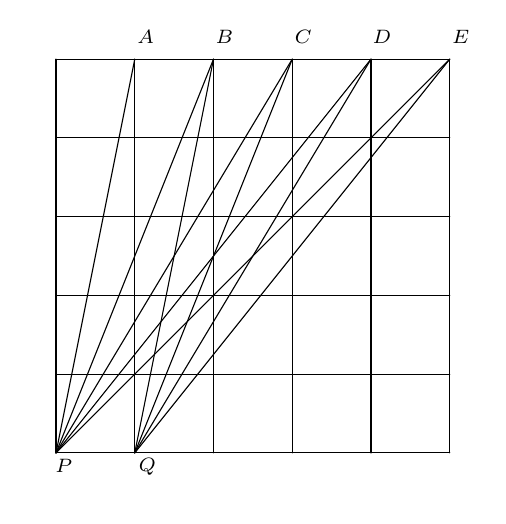
\begin{tikzpicture}[line cap=round,line join=round,>=triangle 45,x=1.0cm,y=1.0cm]
\clip(-2.3600000000000003,-1.540000000000003) rectangle (3.359999999999999,4.3999999999999995);
\draw (-2.0,4.0)-- (3.0,4.0);
\draw (3.0,4.0)-- (3.0,-1.0);
\draw (3.0,-1.0)-- (-2.0,-1.0);
\draw (-2.0,-1.0)-- (-2.0,4.0);
\draw (-1.0,4.0)-- (-1.0,-1.0);
\draw (0.0,-1.0)-- (0.0,4.0);
\draw (1.0,4.0)-- (1.0,-1.0);
\draw (2.0,-1.0)-- (2.0,4.0);
\draw (3.0,3.0)-- (-2.0,3.0);
\draw (-2.0,2.0)-- (3.0,2.0);
\draw (3.0,1.0)-- (-2.0,1.0);
\draw (-2.0,0.0)-- (3.0,0.0);
\draw (-1.0,4.0)-- (-2.0,-1.0);
\draw (-2.0,-1.0)-- (0.0,4.0);
\draw (1.0,4.0)-- (-2.0,-1.0);
\draw (-2.0,-1.0)-- (2.0,4.0);
\draw (3.0,4.0)-- (-2.0,-1.0);
\draw (-1.0,-1.0)-- (0.0,4.0);
\draw (-1.0,-1.0)-- (1.0,4.0);
\draw (-1.0,-1.0)-- (2.0,4.0);
\draw (-1.0,-1.0)-- (3.0,4.0);
\begin{scriptsize}
\draw[color=black] (-1.9000000000000001,-1.1600000000000026) node {$P$};
\draw[color=black] (-0.8400000000000005,-1.1800000000000026) node {$Q$};
\draw[color=black] (3.1399999999999992,4.279999999999999) node {$E$};
\draw[color=black] (2.1399999999999992,4.279999999999999) node {$D$};
\draw[color=black] (1.1399999999999992,4.279999999999999) node {$C$};
\draw[color=black] (-0.8600000000000004,4.279999999999999) node {$A$};
\draw[color=black] (0.1399999999999994,4.279999999999999) node {$B$};
\end{scriptsize}
\end{tikzpicture}
}
\noindent Mennyi a $PAQ\sphericalangle, PBQ\sphericalangle,PCQ\sphericalangle,PDQ\sphericalangle$ és $PEQ\sphericalangle$
szögek összege?
\item Adott egy kocka. A felületére fessünk úgy egy téglalapot, hogy az pontosan a határoló lapok mindegyikének a felét fedje le.
\item Adjunk meg 100 különböző pozitív egész számot úgy, hogy az összegük 5051 legyen.
\item A 2009 számhoz jobbról írjunk hozzá három számjegyet úgy, hogy a kapott hétjegyű szám osztható legyen 7-tel, 9-cel és 11-gyel is.
\item Döntsük el zsebszámológép használata nélkül, hogy 16016003 prímszám-e vagy nem.
\end{enumerate}

\subsection*{2009.02.24.}
\begin{enumerate}
\item Adott a térben 4 nem egy síkba eső pont. Hányféleképpen lehet a 4 ponttól egyenlő távolságra síkokat elhelyezni?
\item Egy 30 fős osztályból hányféleképpen lehet 3 10-fős csapatot alakítani?
\item Hány olyan 1000-nél kisebb egész szám van, amely nem osztható sem 3-mal, sem 5-tel, sem 7-tel?
\item Hány olyan pozitív egész szám van, amely 56~700~000-nál kisebb és hozzá relatív prím?
\item Hányféleképpen lehet a $10^6$-t három tényező szorzatára bontani?
\item Hány megoldása van a pozitív egészek körében az $x+y+z=20$ egyenletnek?
\end{enumerate}

\subsection*{2009.03.04.}
\begin{enumerate}
\item Az ábrán $AB=AC$ és $AP = PQ = QB = BC$. Számítsuk ki az $ABC$ háromszög szögeit.

\centerline{
\definecolor{qqqqff}{rgb}{0.0,0.0,1.0}
\begin{tikzpicture}[line cap=round,line join=round,>=triangle 45,x=1.0cm,y=1.0cm]
%\clip(-0.09999999999999946,-0.28000000000000236) rectangle (2.3000000000000016,4.3999999999999995);
\draw (1.0,4.0)-- (2.0,0.0);
\draw (1.0,4.0)-- (0.0,0.0);
\draw (0.531764705882353,2.127058823529412)-- (1.826297577854671,0.6948096885813155);
\draw (1.826297577854671,0.6948096885813155)-- (0.0,0.0);
\draw (0.0,0.0)-- (2.0,0.0);
\begin{scriptsize}
\draw [fill=qqqqff] (0.0,0.0) circle (1.5pt);
\draw [fill=black] (2.0,0.0) circle (1.5pt);
\draw[color=black] (2.1400000000000015,0.2699999999999978) node {$C$};
\draw [fill=black] (1.0,4.0) circle (1.5pt);
\draw[color=black] (1.240000000000001,3.9) node {$A$};
\draw [fill=black] (0.0,0.0) circle (1.5pt);
\draw[color=black] (-0.1,0.1799999999999978) node {$B$};
\draw [fill=black] (0.531764705882353,2.127058823529412) circle (1.5pt);
\draw[color=black] (0.4200000000000008,2.2999999999999986) node {$P$};
\draw [fill=black] (1.826297577854671,0.6948096885813155) circle (1.5pt);
\draw[color=black] (1.9600000000000013,0.9799999999999981) node {$Q$};
\end{scriptsize}
\end{tikzpicture}
}
\item Határozzuk meg a $6^{2009}$ szám utolsó két számjegyét!
\item Írjuk be a hiányzó számokat a körökbe úgy, hogy bármely szakasz mentén a számok összege 72 legyen.

\centerline{
\begin{tikzpicture}[line cap=round,line join=round,>=triangle 45,x=1.0cm,y=1.0cm]
\clip(-2.38,-0.8800000000000014) rectangle (6.400000000000001,6.700000000000001);
\draw (2.0000000000000004,6.155367074350506)-- (0.0,0.0);
\draw (0.0,0.0)-- (5.23606797749979,3.804226065180613);
\draw (5.23606797749979,3.804226065180613)-- (-1.2360679774997894,3.8042260651806146);
\draw (-1.2360679774997894,3.8042260651806146)-- (4.0,0.0);
\draw (4.0,0.0)-- (2.0000000000000004,6.155367074350506);
\draw[fill=white](2.0000000000000004,6.155367074350506) circle (0.5015974481593778cm);
\draw[fill=white](2.7639320225002106,3.8042260651806123) circle (0.5015974481593778cm);
\draw[fill=white](5.23606797749979,3.804226065180613) circle (0.5015974481593778cm);
\draw[fill=white](1.2360679774997898,3.8042260651806132) circle (0.5015974481593778cm);
\draw[fill=white](-1.2360679774997894,3.8042260651806146) circle (0.5015974481593778cm);
\draw[fill=white](0.7639320225002105,2.3511410091698925) circle (0.5015974481593778cm);
\draw[fill=white](3.2360679774997902,2.351141009169892) circle (0.5015974481593778cm);
\draw[fill=white](2.000000000000001,1.4530850560107216) circle (0.5015974481593778cm);
\draw[fill=white](4.0,0.0) circle (0.5015974481593778cm);
\draw[fill=white](0.0,0.0) circle (0.5015974481593778cm);
\draw (4.860000000000001,3.9000000000000004) node[anchor=north west] {10};
\draw (2.460000000000001,3.9800000000000004) node[anchor=north west] {13};
\draw (3.640000000000001,0.15999999999999892) node[anchor=north west] {14};
\draw (-0.23999999999999944,0.17999999999999894) node[anchor=north west] {19};
\draw (1.720000000000001,1.5799999999999994) node[anchor=north west] {23};
\end{tikzpicture}
}
\item Hány olyan hatjegyű $\overline{abcabc}$ alakú szám van, amely osztható 23-mal?
\item Melyik az a legkisebb prímszám, amely nem állítható elő $2^n$ és $3^k$ alakú számok különbségeként, ahol $n$ és $k$ természetes számok?
\end{enumerate}

\subsection*{2009.04.07.}
\begin{enumerate}
\item Egy iskolai bajnokságban 6 versenyző van. Mindenki mindenki ellen játszik.
Igazoljuk, hogy bármely időpontban vagy van 3 olyan versenyző akik közül mindegyik játszott mindegyikkel, vagy van 3 olyan versenyző, akik közül egyik sem játszott egyikkel sem.
\item Egy konvex sokszögben összesen 77 átló van. Hány oldalú a sokszög?
\item Hány olyan háromjegyű szám van, amelyben csak két különböző számjegy szerepel?
\item Az 1, 2, 3, 4, 5 számjegyekből hány olyan négyjegyű szám képezhető, amelyben legalább egy számjegy ismétlődik?
\item Az 1, 2, 3, 4, 5, 6, 7 számjegyekből készített ötjegyű számok közül hányban fordul elő az 1 számjegy, ha egy számban minden számjegy legfeljebb egyszer szerepelhet?
\end{enumerate}

\subsection*{2009.05.26.}
\begin{enumerate}
\item A $\dfrac{3n+2}{4n+1}$ tört ($n\ge 1$, egész) mely $n$-ekre egyszerűsíthető?
\item Igazoljuk, hogy ha $n\ge 1$ egész, akkor $\left(2^n+1; 2^n-1\right)=1$.
\item Legyen $A=11111111$ és $B=\underbrace{11\ldots 11}_{100\text{~db}}$. Határozzuk meg $A$ és $B$ legnagyobb közös osztóját!
\item Melyik az a háromjegyű szám, amelyből 6-ot elvéve 7-tel osztható, 7-et elvéve 8-cal osztható, 8-cat elvéve 9-cel osztható számot kapunk?
\item Van-e 3 olyan egymástól különböző pozitív egész, amelyek négyzetének összege négyzetszám?
\item Igazoljuk, hogy nincs olyan 11 egymást követő egész, amelyek négyzetének összege négyzetszám.
\end{enumerate}
\end{document}
